\documentclass[format=acmlarge]{acmart}

\usepackage{amsmath}
\DeclareMathOperator*{\argmax}{argmax}

\usepackage{hyperref}

\setcopyright{rightsretained}
\copyrightyear{2017}

\begin{document}
\title{Survey of machine learning techniques over a course of study}

\author{Kenneth Allen}
\affiliation{%
  \institution{Armstrong State University}
  \department{Department of Computer Science \& Information Technology}
  \city{Savannah}
  \state{GA}
  \postcode{31419}
  \country{United States of America}}
\email{ka3878@stu.armstrong.edu}

\author{Jeffrey Young}
\affiliation{%
  \institution{Armstrong State University}
  \department{Department of Computer Science \& Information Technology}
  \city{Savannah}
  \state{GA}
  \postcode{31419}
  \country{United States of America}}
\email{jy8672@stu.armstrong.edu}

\begin{abstract}
Machine learning is the problem of extrapolating the approximation of a function from a limited, often noisy set of training values.  There are many techniques that can be used to achieve results in this domain, some areas of active research and some primarily of theoretical interest.  We describe three of the most prominent machine learning techniques and our experience using them to classify data in two different domains.
\end{abstract}

\keywords{Machine learning, Neural networks, Neuroph, Stock prediction, S\&P 500, Text classification, Naive Bayes\"{i}an, Headlines, Support vector machines, LibSVM}

\maketitle

\section{Methods}
\subsection{Na\"{i}ve Bayesian}
A Bayesian classifier is based on the idea that the role of a (natural) class is to predict the values of features for members of that class. Examples are grouped in classes because they have common values for the features.  The na\"{i}ve assumption of class-conditional independence is often made, given

$$P(X|C_i) = \prod_{k = 1}^n P(x_k|C_i) .$$

\subsection{Support Vector Machine}
A Support Vector Machine (SVM) is a discriminative classifier formally defined by a separating hyperplane. In other words, given labeled training data (supervised learning), the algorithm outputs an optimal hyperplane which categorizes new examples. For example, in a two-dimensional space, the hyperplane is a line dividing the plane into two parts with each class positioned in either part, as in Fig. 1.

\begin{figure}
  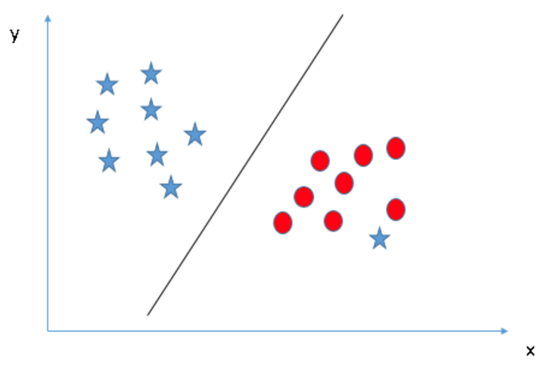
\includegraphics{svm-example}
  \caption{Support vector machine example, with hyperplane separating examples.}
  \label{fig:one}
\end{figure}

\subsection{Neural Network}
An Artificial Neural Network (ANN) is an information processing paradigm that is inspired by the way biological nervous systems, such as the brain, process information. The key element of this paradigm is the novel structure of the information processing system. It is composed of a large number of highly interconnected processing elements (neurons) working in unison to solve specific problems. ANNs, like people, learn by example. An ANN is configured for a specific application, such as pattern recognition or data classification, through a learning process. ANNs can theoretically approximate any function to arbitrary accuracy.

Feed-forward neural networks are the simplest type, organized into discrete layers that only feed from the preceding layer and into the proceeding one.

\begin{figure}
  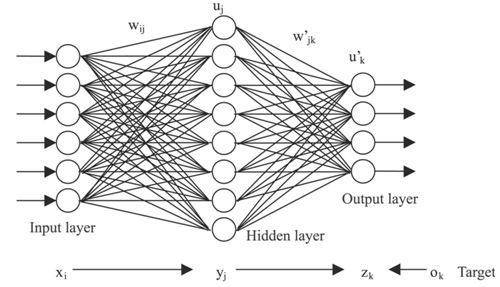
\includegraphics{nn-example}
  \caption{Neural network example, with neurons and links between layers.}
  \label{fig:two}
\end{figure}

\section{Results}
We compare and contrast our experiences working with the classifier types, with numerical results summarized in Table 1.  It should be kept in mind that results from different domains cannot be compared directly.

\begin{table}
  \caption{Best results of classifiers of different types.}
  \label{tab:one}
  \begin{tabular}{lllll}
    Technique & Domain & Accuracy & $F_1$ score & ROC-AUC\\
    \hline
    Na\"{i}ve Bayesian & Classifying headlines by origin publication & 0.931 & 0.953 & 0.912\\
    SVM & Classifying stocks by performance & 0.820 & 0.824 & 0.821\\
    Neural network & Classifying stocks by performance & 0.800 & 0.792 & 0.892\\
  \end{tabular}
\end{table}

\subsection{Na\"{i}ve Bayesian: Headlines}
Bayesian classification was simple enough that we implemented it in code ourselves.  We took what we thought would be a difficult task of classifying simply based on word counts in headlines where an article originated.  The two publications had different national and demographic audiences, and differences in diction and style proved a fairly reliable way to distinguish them.  Simple to code, without parameters to tune, and fast to train and evaluate, na\"{i}ve Bayesian classifiers have usefulness in certain domains where the volume of data is greater than its complexity or subtlety.

\subsection{SVM: Stock Returns}
We used LibSVM to calculate and evaluate our classifier.  We tuned by measuring results with a variety of different kernels, kernel parameters, and error penalty ($C$) values, getting best performance from a quartic kernel and a very low $C$ value (0.25).  It was able to correctly predict whether a stock's returns would beat the market average in the following year 82\% of the time.  With our large feature set, optimizing and evaluating the classifier took a significant amount of time.  The results were promising, but tuning the SVM requires expertise or brute computing force.  Some of our more outlandish configurations produced wildly divergent results, so caution is advised.

\subsection{Neural Network: Stock Returns}
We used the Neuroph library to train and evaluate our classifier.  One issue with neural networks is that, with randomized starting weights, their training is nondeterministic from execution to execution, subject to becoming 'trapped' in local minima on the error surface.  The primary parameter to tune is the number of and size of its hidden layers; after testing multiple options, we settled on a single hidden layer of 30 neurons.  Backpropagation training takes a significant amount of time and is tricky to parallelize effectively on data like ours, but the results were comparable with the SVM on the same data (80\% accuracy).  Because neural network classifiers have a tunable sensitivity/strictness parameter, the area under the curve for the Receiver Operating Characteristic (ROC-AUC) was significantly above that of the SVM classifier.

\section{Conclusion}
All three of the machine learning techniques we studied this semester have applicability to certain domains.  Na\"{i}ve Bayesian is computationally cheap and simple for the results it can produce.  SVMs are a useful tool if an expert is available to tune them properly, and neural networks can be made arbitrarily accurate with more neurons and layers, although both of these require significant computing power.  They are each an important tool in the data scientist's toolkit.

\section{Works Cited}
\begin{itemize}
  \item Stergiou, C., \& Siganos, D. (n.d.). \textit{NEURAL NETWORKS}. Retrieved December 08, 2017, from http://www.doc.ic.ac.uk/~nd/surprise\_96/journal/vol4/cs11/report.html\#What\%20is\%20a\%20Neural\%20Network
  \item Patel, S. (2017, May 03). \textit{Chapter 2 : SVM (Support Vector Machine) - Theory - Machine Learning 101}. Retrieved December 08, 2017, from https://medium.com/machine-learning-101/chapter-2-svm-support-vector-machine-theory-f0812effc72
  \item \textit{Artificial Intelligence}. (n.d.). Retrieved from http://artint.info/html/ArtInt\_181.html
\end{itemize}

\end{document}